%
%===============>>  ГРУППА 7-1 МОДУЛЬ 7  <<=============
%
\setmodule{7}

%BEGIN_FOLD % ====>>_____ Занятие 1 _____<<====
\begin{class}[number=1]
	\begin{definit}
		Если секущая пересекает две параллельные прямые, то:
		\begin{tasks}(1)
			\task внутренние накрест лежащие углы равны: \( \angle 4 \) и \( \angle5 \), \( \angle 3 \) и \( \angle 6\);
			\task сумма внутренних односторонних углов равна  \(180\degree\): \( \angle 3 \) и \( \angle 5 \), \( \angle 4 \) и \( \angle 6 \);
			\task соответственные углы равны: \( \angle 1 \) и \( \angle 5 \), \( \angle 2 \) и \( \angle 6 \), \( \angle 3 \) и \( \angle 7 \), \( \angle 4 \) и \( \angle 8 \);
			\task внешние накрест лежащие углы равны: \( \angle 2 \) и \( \angle 7 \), \( \angle 1 \) и \( \angle 8 \);
			\task сумма внешних односторонних углов равна  \(180\degree\): \( \angle 1 \) и \( \angle 7 \), \( \angle 2 \) и \( \angle 8 \).
		\end{tasks}
		\begin{minipage}[c]{0.9\linewidth}
			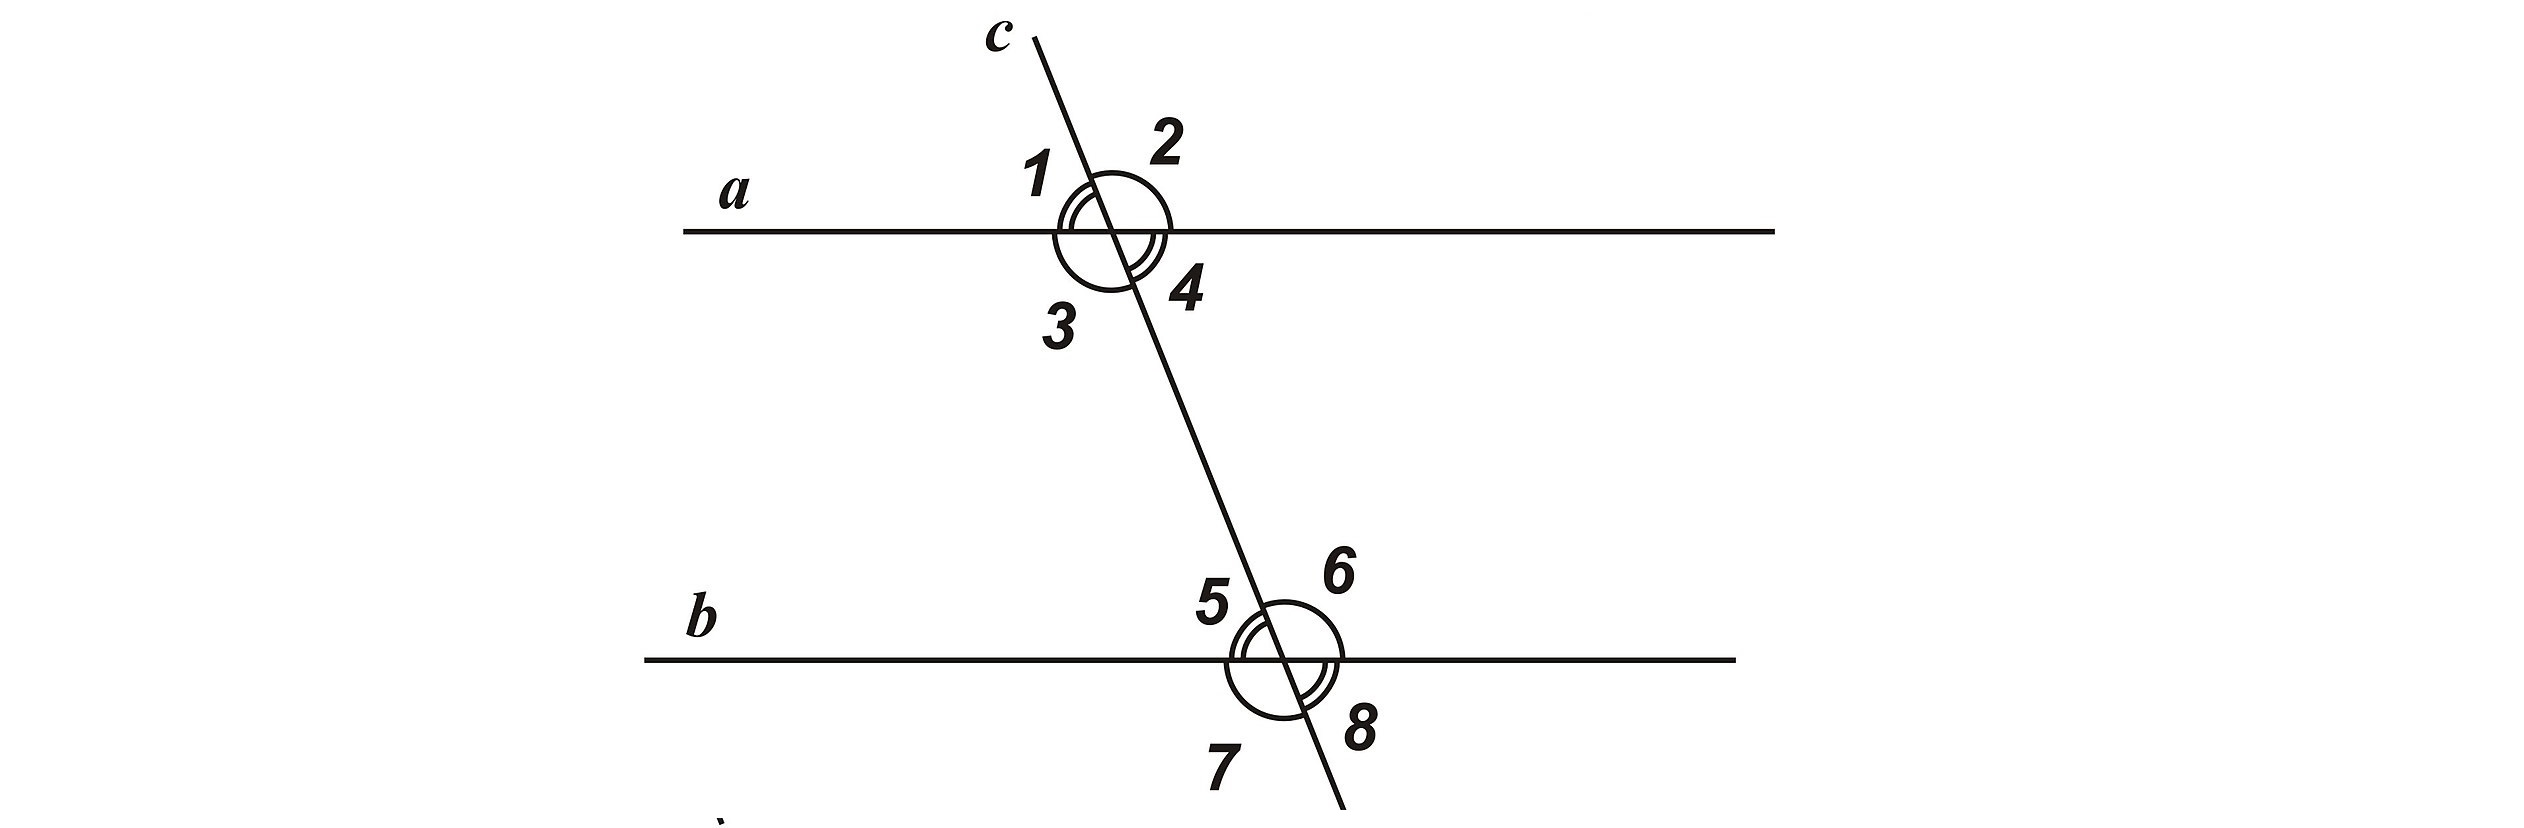
\includegraphics[align=t, width=\linewidth]{\picpath/sorokinM6L1-1}
		\end{minipage}
	\end{definit}
	\begin{listofex}
		\item Сумма накрест лежащих углов при пересечении двух параллельных прямых и секущей равна \(210 \degree \). Найдите эти углы.
		\item Найдите все углы, образованные при пересечении параллельных прямых \(a\) и \(b\) с секущей \(c\), если один из углов равен \( 150 \degree \).
		\item Через вершину \(C\) треугольника \(ABC\) проведена прямая, параллельная биссектрисе \(BD\) угла \(ABC\). Эта прямая пересекает прямую \(AB\) в точке \(K\). Найдите углы треугольника \(BKC\), если \(\angle ABC = 130 \degree\).
		\item Через вершину \(B\) треугольника \(ABC\) проведена прямая, параллельная прямой \(AC\). Образовавшиеся при этом три угла с вершиной B относятся как \(3 : 10 : 5\). Найдите углы треугольника \(ABC\).
		%\item Через середину \(M\) отрезка с концами на двух параллельных прямых проведена прямая, пересекающая эти прямые в точках \(A\) и \(B\). Докажите, что \(M\) также середина \(AB\).
		%\item Внешние углы треугольника \(ABC\) при вершинах \(A\) и \(C\) равны \(115\degree\) и \(140\degree \). Прямая, параллельная прямой \(AC\), пересекает стороны \(AB\) и \(AC\) в точках \(M\) и \(N\). Найдите углы треугольника \(BMN\).
		%\item Через точку \(M\), лежащую внутри угла с вершиной \(A\), проведены прямые, параллельные сторонам угла и пересекающие эти стороны в точках \(B\) и \(C\). Известно, что \(\angle ACB = 50\degree\), а угол, смежный с углом \(ACM\), равен \(40\degree\). Найдите углы треугольников \(BCM\) и \(ABC\).
		%\item Прямая пересекает боковую сторону \(AC\), основание \(BC\) и продолжение боковой стороны \(AB\) равнобедренного треугольника \(ABC\) за точку \(B\) в точках \(K, L\) и \(M\) соответственно. При этом треугольники \(CKL\) и \(BML\) получаются также равнобедренными. Найдите их углы.
		%\item Отрезки \(AB\) и \(CD\) пересекаются в точке \(O\) и делятся этой точкой пополам. Докажите, что \(AC \parallel BD, AD \parallel BC\).
		%\item Точки \(A\) и \(D\) лежат на одной из двух параллельных прямых, точки \(B\) и \(C\) --- на другой, причем прямые \(AB\) и \(CD\) также параллельны. Докажите, что противоположные углы четырехугольника \(ABCD\) равны между собой.
	\end{listofex}
\end{class}
%END_FOLD

%BEGIN_FOLD % ====>>_____ Занятие 2 _____<<====
\begin{class}[number=2]
	\begin{listofex}
		\item Через середину \(M\) отрезка с концами на двух параллельных прямых проведена прямая, пересекающая эти прямые в точках \(A\) и \(B\). Докажите, что \(M\) также середина \(AB\).
		\item Внешние углы треугольника \(ABC\) при вершинах \(A\) и \(C\) равны \(115\degree\) и \(140\degree \). Прямая, параллельная прямой \(AC\), пересекает стороны \(AB\) и \(AC\) в точках \(M\) и \(N\). Найдите углы треугольника \(BMN\).
		\item Через точку \(M\), лежащую внутри угла с вершиной \(A\), проведены прямые, параллельные сторонам угла и пересекающие эти стороны в точках \(B\) и \(C\). Известно, что \(\angle ACB = 50\degree\), а угол, смежный с углом \(ACM\), равен \(40\degree\). Найдите углы треугольников \(BCM\) и \(ABC\).
		\item Прямая пересекает боковую сторону \(AC\), основание \(BC\) и продолжение боковой стороны \(AB\) равнобедренного треугольника \(ABC\) за точку \(B\) в точках \(K, L\) и \(M\) соответственно. При этом треугольники \(CKL\) и \(BML\) получаются также равнобедренными. Найдите их углы.
		\item Отрезки \(AB\) и \(CD\) пересекаются в точке \(O\) и делятся этой точкой пополам. Докажите, что \(AC \parallel BD, AD \parallel BC\).
		\item Точки \(A\) и \(D\) лежат на одной из двух параллельных прямых, точки \(B\) и \(C\) --- на другой, причем прямые \(AB\) и \(CD\) также параллельны. Докажите, что противоположные углы четырехугольника \(ABCD\) равны между собой.
		
		%\item 
		%\begin{minipage}[t]{\bodywidth}
		%	
		%\end{minipage}
		%\hspace{0.02\linewidth}
		%\begin{minipage}[t]{\picwidth}
		%	\includegraphics[align=t, width=\linewidth]{\picpath/}
		%\end{minipage}
	\end{listofex}
\end{class}
%END_FOLD

%BEGIN_FOLD % ====>>_ Домашняя работа 1 _<<====
\begin{homework}[number=1]
	\begin{listofex}
		
		%\item Через точку \(M\), лежащую внутри угла с вершиной \(A\), проведены прямые, параллельные сторонам угла и пересекающие эти стороны в точках \(B\) и \(C\). Известно, что \(\angle ACB = 72\degree\), а угол, смежный с углом \(ACM\), равен \(28\degree\). Найдите углы треугольников \(BCM\) и \(ABC\).
		
		\item Прямая \(CM\) пересекает прямую \(BC\) в точке \(C\) так, что \(BD \parallel CM\). Известно, что \(BD=BC, DB \parallel MC, \angle BCM = 166 \degree\). Найдите угол \( BDC \).
		\item При пересечении двух прямых с секущей один из внутренних углов оказался равен \(135\degree\). Найдите все углы, которые образовались при пересечении прямых.
		\item Внешние углы треугольника \(ABC\) при вершинах \(A\) и \(C\) равны \(145\degree\) и \(110\degree \). Прямая, параллельная прямой \(AC\), пересекает стороны \(AB\) и \(AC\) в точках \(M\) и \(N\). Найдите углы треугольника \(BMN\).
		\item Две параллельные прямые пересечены третьей. Найдите угол между биссектрисами внутренних односторонних углов.
	\end{listofex}
\end{homework}
%END_FOLD

%BEGIN_FOLD % ====>>_____ Занятие 3 _____<<====
\begin{class}[number=3]
	\begin{listofex}
		\item Через середину \(M\) отрезка с концами на двух параллельных прямых проведена прямая, пересекающая эти прямые в точках \(A\) и \(B\). Докажите, что \(M\) также середина \(AB\).
		\item \(AD\) --- биссектриса треугольника \(ABC\). Точка \(M\) лежит на стороне \(AB\), причем \(AM = MD\). Докажите, что \(MD \parallel AC\).
		\item Прямая пересекает параллельные прямые \(a\) и \(b\) в точках \(A\) и \(B\) соответственно. Биссектриса одного из образовавшихся углов с вершиной \(B\) пересекает прямую \(a\) в точке \(C\). Найдите \(AC\), если \(AB = 1\).
		\item На сторонах \(AC\) и \(BC\) треугольника \(ABC\) взяты соответственно точки \(M\) и \(N\), причем \(MN \parallel AB\) и \(MN = AM\). Найдите угол \(BAN\), если \( \angle B = 45 \degree, \angle C = 60 \degree  \).
		
	\end{listofex}
\end{class}
%END_FOLD

%BEGIN_FOLD % ====>>_____ Занятие 4 _____<<====
\begin{class}[number=4]
	\begin{listofex}
		\item Найдите все углы, образованные при пересечении двух параллельных прямых \(a\) и \(b\) и секущей \(c\), если один из углов на \(70 \degree\) больше другого. %203 Геом7-9
		\item Разность двух односторонних углов при пересечении двух параллельных прямых секущей равна \(50 \degree\). Найдите эти углы.
		\item Дана незамкнутая ломаная \(ABCD\), причем \(AB = CD\) и \(\angle ABC = \angle BCD \). Докажите, что \(AD \parallel BC\).
		%\item Равные отрезки \(AB\) и \(CD\) пересекаются в точке \(K\). Известно, что \(AC \parallel BD \). Докажите, что треугольники \(AKC\) и \(BKD\) равнобедренные.
		%\item Концы отрезка \(AB \) лежат на параллельных прямых \(a\) и \(b\). Прямая, проходящая через середину \(O\) этого отрезка пересекает прямые \(a\) и \(b\) в точках \(C\) и \(D\). Докажите, что \(CO=OD\). %204
		%\item Угол \(ABC\) равен \(70 \degree\), а угол \(BCD\) равен \(110 \degree\). Могут ли прямые \(AB\) и \(CD\) быть: параллельными? пересекающимися? %206
		\item Упростите выражение и найдите его значение:
		\begin{tasks}
			\task \( \dfrac{a^2+4a}{a^2+8a+16} \) при \(a=-2\)
			\task \( 0,5 \cdot \dfrac{4b^2+12b+9}{b+1,5} \) при \(b=-5\)
		\end{tasks}
	\end{listofex}
\end{class}
%END_FOLD

%BEGIN_FOLD % ====>>_ Домашняя работа 2 _<<====
\begin{homework}[number=2]
	\begin{listofex}
		\item Найдите все углы, образованные при пересечении двух параллельных прямых \(a\) и \(b\) и секущей \(c\), если один из углов равен \(150 \degree\). %203 Геом7-9
		\item Сумма двух соответствующих углов при пересечении двух параллельных прямых секущей равна \(120 \degree\). Найдите все углы, образованные при пересечении параллельных прямых с секущей.
		\item Внешние углы треугольника \(ABC\) при вершинах \(A\) и \(C\) равны \(150\degree\) и \(105\degree \). Прямая, параллельная прямой \(AC\), пересекает стороны \(AB\) и \(AC\) в точках \(M\) и \(N\). Найдите углы треугольника \(BMN\).
	\end{listofex}
\end{homework}
%END_FOLD

%BEGIN_FOLD % ====>>_____ Занятие 5 _____<<====
\begin{class}[number=5]
	\begin{definit}
	\textbf{Внешний угол} --- угол между стороной треугольника и продолжением другой стороны. Внешний угол является смежным с одним из внутренних.
	\end{definit}
	\begin{listofex} %Взял у Сорокина
		\item В треугольнике \( ABC \) два угла равны \( 50\) и \( 70 \) градусов. Найдите третий угол.
		\item Один угол треугольника равен \( 26\degree \), а второй в три раза больше. Найдите третий угол.
		\item Один внутренний угол треугольника в два, а второй в три раза больше третьего, найдите все углы треугольника.
		\item Один внешний угол равен \( 150\degree \), а второй в \( \dfrac{ 3 }{ 5 } \) раза больше. Чему равны внутренние углы треугольника?
		\item Угол \(ABC\) равен \(70 \degree\), а угол \(BCD\) равен \(110 \degree\). Могут ли прямые \(AB\) и \(CD\) быть: параллельными? пересекающимися? %206
		\item Угол треугольника равен \( 30\degree \), второй угол в \( 3 \) раза больше первого. Чему равны внешние углы при каждой вершине? Чему равна сумма внешних углов? Как называется такой треугольник?
		%\item Равные отрезки \(AB\) и \(CD\) пересекаются в точке \(K\). Известно, что \(AC \parallel BD \). Докажите, что треугольники \(AKC\) и \(BKD\) равнобедренные.
		\item Концы отрезка \(AB \) лежат на параллельных прямых \(a\) и \(b\). Прямая, проходящая через середину \(O\) этого отрезка пересекает прямые \(a\) и \(b\) в точках \(C\) и \(D\). Докажите, что \(CO=OD\). %204
		\item Найдите значение выражения при заданных значениях переменной:
		\begin{tasks}(2)
			\task \( \dfrac{(x)^7}{(x^3)^2} \) при \( x=-\dfrac{5}{2} \)
			\task \( \dfrac{(4y)^3}{(8y)^5} \) при \( y=5 \)
			\task \( \dfrac{(10a)^3 \cdot (a)^5}{(a^4)^2} \) при \( a=-0,25231 \)
			\task \( \dfrac{(4c)^5 \cdot (2c)^6}{(4c)^2} \) при \( c=-0,5 \)
		\end{tasks}
		
	\end{listofex}
\end{class}
%END_FOLD

%BEGIN_FOLD % ====>>_____ Занятие 6 _____<<====
\begin{class}[number=6]
	\begin{listofex}
		\item Точки \(A\) и \(C\) лежат по одну сторону от прямой \(a\). Перпендикуляры \(AB\) и \(CD\) к прямой \(a\) равны. % 105
		\begin{tasks}
			\task Докажите, что \( \angle ABD = \angle CDB \),
			\task Найдите  \( \angle ABC \), если \( \angle ADB =44 \degree \).
		\end{tasks}
		\item 
		\begin{minipage}[t]{\bodywidth}
			Докажите, что треугольники \(TCO\) и \( BOP \) равны.
		\end{minipage}
		\hspace{0.02\linewidth}
		\begin{minipage}[t]{\picwidth}
			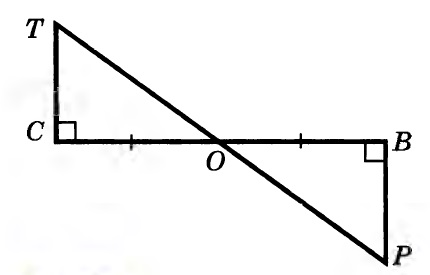
\includegraphics[align=t, width=\linewidth]{\picpath/G71M7L6-1}
		\end{minipage}
		\item %187
		\begin{minipage}[t]{\bodywidth}
			По данным рисунка докажите, что \(AB \parallel DE\).
		\end{minipage}
		\hspace{0.02\linewidth}
		\begin{minipage}[t]{\picwidth}
			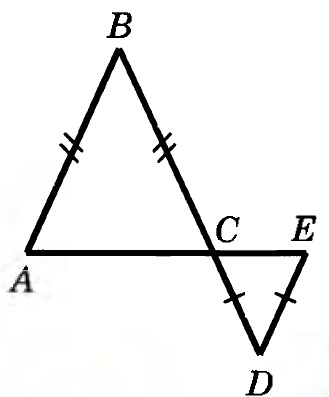
\includegraphics[align=t, width=\linewidth]{\picpath/G71M7L6-2}
		\end{minipage}
		\item В треугольнике \(ABC\) угол \(A\) равен \(40 \degree\), а угол \(BCE\), смежный с углом \(ABC\), равен \(80 \degree\). Докажите, что биссектриса угла \(BCE\) параллельна \(AB\). %192
		
		%191
		\item Отрезок \(BK\) --- биссектриса треугольника \(ABC\). Через точку \(K\) проведена прямая, пересекающая сторону \(BC\) в точке \(M\) так, что \(BM=MK\). Докажите, что \(KM \parallel AB\). 
		\item На сторонах вертикальных углов отложены от его вершины равные отрезки \(OA, OB, OC\) и \(OD\). Укажите пары равных треугольников с вершинами в точках \(O, A, B, C\) и \(D\).
		%190
		\item 
		\begin{minipage}[t]{\bodywidth}
			На рисунке \(AB=BC, AD=DE, \angle C = 70 \degree, \angle EAC = 35 \degree\). Докажите, что \(DE \parallel AC\)
		\end{minipage}
		\hspace{0.02\linewidth}
		\begin{minipage}[t]{\picwidth}
			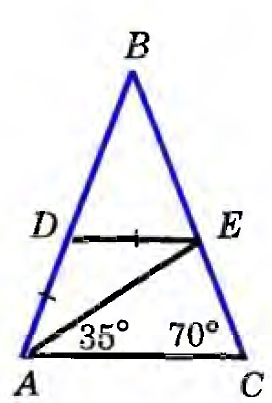
\includegraphics[align=t, width=\linewidth]{\picpath/G71M7L6-3}
		\end{minipage}
	\end{listofex}
\end{class}
%END_FOLD

%BEGIN_FOLD % ====>>_ Домашняя работа 3 _<<====
\begin{homework}[number=3]
	\begin{listofex}
		%107
		\item В равнобедренном треугольнике основание в два раза меньше боковой стороны, а периметр равен \(50\) см. Найдите стороны треугольника.
		\item Внешние углы треугольника \(ABC\) при вершинах \(A\) и \(C\) равны \(115\degree\) и \(140\degree \). Прямая, параллельная прямой \(AC\), пересекает стороны \(AB\) и \(AC\) в точках \(M\) и \(N\). Найдите углы треугольника \(BMN\).
		\item Через точку \(M\), лежащую внутри угла с вершиной \(A\), проведены прямые, параллельные сторонам угла и пересекающие эти стороны в точках \(B\) и \(C\). Известно, что \(\angle ACB = 50\degree\), а угол, смежный с углом \(ACM\), равен \(40\degree\). Найдите углы треугольников \(BCM\) и \(ABC\).
		%193
		\item В треугольнике \( ABC, \angle A = 40 \degree, \angle B = 70 \degree \). Через вершину \(B\) проведена прямая \(BD\) так, что \(BC\) --- биссектриса угла \(ABD\). Докажите, что \(AC \parallel BD\).
	\end{listofex}
\end{homework}
%END_FOLD

%BEGIN_FOLD % ====>>_____ Занятие 7 _____<<====
\begin{class}[number=7]
	\title{Подготовка к проверочной}
	\begin{listofex}
		\item Занятие 7
	\end{listofex}
\end{class}
%END_FOLD

=%BEGIN_FOLD % ====>>_ Проверочная работа _<<====
\begin{exam}
	\begin{listofex}
		\item Проверочная
	\end{listofex}
\end{exam}
%END_FOLD